\documentclass[a4paper,12pt]{article}
\setlength\textwidth{7in}
\usepackage{amssymb,amsmath}
\usepackage{verbatim,graphicx}
\usepackage{fullpage}
\begin{document}

	\begin{titlepage}

		\vspace*{2cm}
		\begin{center}
            \large{\textbf{Comparison of Intrusion Detection Systems based on Machine Learning and Data Mining Algorithms for Low-Powered Devices}}
		\end{center}
		\vspace{0.5cm}
		\begin{center}
            \small{\textit{Project progress report submitted} \\ \vspace{0.25cm} \textit{to} \\ \vspace{0.25cm}\textbf{MANIPAL ACADEMY OF HIGHER EDUCATION} \\}
		\end{center}
		\vspace{0.25cm}
		\begin{center}
		\small{\textit{For Partial Fulfillment of the Requirement for the\\ \vspace{0.25cm}Award of the Degree\\ \vspace{0.25cm}of}} \\ \vspace{0.25cm}
		\textbf{Bachelor of Technology} \\  \vspace{0.25cm} \textit{in} \\ \textbf{Computer and Communication Engineering}
		\end{center}
		\begin{center}
		\small{\textit{by}} \\
		\textbf{Pratyay Amrit} \\ \textbf{Reg. No. 140953430} \\
		\end{center}

		\begin{center}
		\small{\textit{Under the guidance of}} \\
		\renewcommand{\baselinestretch}{1}
		\vspace{0.5cm}
		Ms. Ipsita Upasana \\
		Assistant Professor \\
		Department of I \& CT \\
		 Manipal Institute of Technology \\
		Manipal, India
		\end{center}

		\begin{figure}[h]
	  	\begin{center}
		
\includegraphics{MITLogo}
		\end{center}
		\end{figure}
		\begin{center}
		\textbf{Jan 2018}
		\end{center}

	\end{titlepage}

	%\newpage

	\newpage

	\section{Introduction}
	\paragraph{}
	Security in low-powered devices has always been a major concern as their limited computational capacity prohibits the use of sophisticated algorithms. An Intrusion Detection System(IDS) provides a first-line monitoring service for the devices to help them protect themselves against anomalous data. Several methods have been proposed to implement such a system, ranging from Association Rule Mining to complex Machine Learning algorithms. Most of these systems, however, fail to address the issue of low computational capabilities of small devices, which may soon comprise the majority of man-machine interaction with the ever growing popularity of IoT. This work attempts to analyze and compare the performance of some of these methods. UNSW-NB15 dataset has been used for testing these methods. The KDD'99 dataset has been popular for the development of such systems, however, the dataset has a few problems. UNSW-NB15 is a recently curated dataset that has been gaining popularity in recent years. It provides a more modern set of data and features to be used in IDSs for detecting modern attacks. It also addresses some of the issues in KDD'99 \cite{unsw15}.

	\section{Problem Definition}
	\paragraph{}
	Technology is growing rapidly every day, and so are incidents concerned with cyber security. Intrusion Detection Systems are responsible for monitoring the network and detecting a data packet that may pose a risk for the network. Primitive IDSs were built to detect attacks on the basis of their signature. Every time a new attack was discovered, it's signature was recorded to protect the system from similar future attacks. This, however, could not prevent the system from new attacks. With the advent of Machine Learning and Data Mining techniques, these IDSs could now be taught how an attack looks in the network to perform detection of new attacks. This however, significantly increased the false positives in detection. Another problem came up as IoT began expanding exponentially. Massive networks of small, low-powered devices have taken over the majority of space in todays world. These small devices, however, lack the ability to execute complicated machine learning algorithms. This work attempts to assess the performance of some of these algorithms in such low powered devices.

	\section{Objective}
    The objectives of this work can be summarized as follows:
	\begin{enumerate}
		\item To find and choose a dataset that will resemble a network dump as closely as possible, and must conform with modern trends to make sure the IDS is well trained for novel attacks.
		\item To develop IDSs based on \cite{dm15} and \cite{mlp17}. These works propose two very popular classification algorithms, K-Means and Multilayer Perceptron respectively.
		\item To analyze and compare the two algorithms based on similar parameters. The accuracy and efficiency of these algorithms must be taken in to account.
		\item To test these algorithms in low powered devices and compare the effects of the decreased computational power.
		\item To make an attempt to scale down the complexity of these algorithms to make it more efficient for low powered devices.
        \item To analyze the optimized algorithms and compare them
	\end{enumerate}

	\section{Scope}
	\paragraph{}
	This work will benefit cyber security companies or agencies to understand how different types of IDS perform on similar environments and may use this work to influence their decision in choosing one. This work will help individuals working in IoT or cyber security domain in making the right choice for their specific scenarios. This work may also help future research in developing an all round hybrid IDS capable of performing equally well in both, high end and low powered devices, as well as analyzing and comparing other numerous algorithms used for developing Intrustion Detection Systems.

	\section{Literature Survey}
	\paragraph{}
    \cite{unsw15} is a comparative study of the two most popular datasets used for testing Intrusion Detection Systems. It explains the shortcomings of the KDD'99 dataset while introducing the UNSW-NB15 dataset. In this paper, the feature characteristics of the UNSW-NB15 and KDD'99 datasets are examined, and the features of the UNSW-NB15 are replicated to the KDD99 data set to measure their effeciency, they apply An Association Rule Mining algorithm as feature selection to generate the strongest features from the two datasets.
    \paragraph{}
	\cite{dm15} proposes the use of k-means algorithm for IDS. The algorithm is tested with various number of clusters and the best result was shown to be when the number of clusters equalled 22 for the static database the algorithm was tested with. In a dynamic network, however, the number of clusters will greatly affect the results for different data sets and thus, identifying the number of clusters becomes an important issue.
	\paragraph{}
	\cite{mlp17} proposes the use of multi-layer perceptrons for building an IDS. The model performs better than other methods, however, is computationally expensive. The authors lowered the computational load by binarizing the weights on the neural network. This allowed the use of this algorithm in low powered devices, but also resulted in a drop in performance by 4 times.

	\section{Methodology}
        \subsection{Dataset}
            \paragraph{}
                The UNSW-NB15 dataset has recently been released. It was generated using tcpdump tool to capture 100GB of raw data. It has the following 9 types of attacks:
                \begin{enumerate}
                    \item Fuzzers: Fuzzing, or Fuzz Testing is a black box testing technique in which aims at finding implementation bugs by injecting malformed or semi-malformed data in an automated fashion. Potential attackers may run fuzz tests on the network to find vulnerabilities that can be exploited.
                    \item Analysis: Traffic analysis is a special type of inference attack technique that looks at communication patterns between entities in a system. Knowing who's talking to whom, when, and for how long, can sometimes clue an attacker in to information of which you'd rather she not be aware.
                    \item Backdoor: A backdoor is a malware type that negates normal authentication procedures to access a system.
                    \item DoS: Denial of Service (DoS) is an attack which aims to make a host machine unavailable to its intended users by temporarily or indefinitely disrupting the host machines connection to the internet.
                    \item Exploit: An exploit is a piece of software, a chunk of data, or a sequence of commands that takes advantage of a bug or vulnerability to cause unintended or unanticipated behavior to occur on computer software, hardware, or something electronic.
                    \item Generic: This subset contains any general type of attack such as probe, u2r, r2l etc.
                    \item Reocinnaissance: Active reconnaissance is a type of computer attack in which an intruder engages with the targeted system to gather information about vulnerabilities.
                    \item Shellcode: A shellcode is a small piece of code used as the payload in the exploitation of a software vulnerability.
                    \item Worm: A computer worm is a standalone malware computer program that replicates itself in order to spread to other computers. Often, it uses a computer network to spread itself, relying on security failures on the target computer to access it.
                \end{enumerate}
            \paragraph{}
            The dataset contains 2,540,044 records with 49 features categorized into 6 categories.
            \begin{enumerate}
                \item \textbf{Flow Features:} \\
                    1. srcip: Source IP address. \\
                    2. sport: Source port number. \\
                    3. dstip: Destinations IP address. \\
                    4. dsport: Destination port number. \\
                    5. proto: Protocol type, such as TCP, UDP.
                \item \textbf{Basic Features:} \\
                    6. state: The states and its dependent protocol e.g., CON. \\
                    7. dur: Row total duration. \\
                    8. sbytes: Source to destination bytes. \\
                    9. dbytes: Destination to source bytes. \\
                    10. sttl: Source to destination time to live. \\
                    11. dttl: Destination to source time to live. \\
                    12. sloss: Source packets retransmitted or dropped. \\
                    13. dloss: Destination packets retransmitted or dropped. \\
                    14. service: Such as http, ftp, smtp, ssh, dns and ftp-data. \\
                    15. sload: Source bits per second. \\
                    16. dload: Destination bits per second. \\
                    17. spkts: Source to destination packet count. \\
                    18. dpkts: Destination to source packet count.
                \item \textbf{Content Features:} \\
                    19. swin: Source TCP window advertisement value. \\
                    20. dwin: Destination TCP window advertisement value. \\
                    21. Stcpb: Source TCP base sequence number. \\
                    22. dtcpb: Destination TCP base sequence number. \\
                    23. smeansz: Mean of the packet size transmitted by the srcip. \\
                    24. dmeansz: Mean of the packet size transmitted by the dstip. \\
                    25. trans\_depth: The connection of http request/response transaction. \\
                    26. res\_bdy\_len: The content size of the data transferred from http.
                \item \textbf{Time Features:} \\
                    27. sjit: Source jitter. \\
                    28. djit: Destination jitter. \\
                    29. stime: Row start time. \\
                    30. ltime: Row last time. \\
                    31. sintpkt: Source inter-packet arrival time. \\
                    32. dintpkt: Destination inter-packet arrival time. \\
                    33. tcprtt: Setup round-trip time, the sum of ’synack’ and ’ackdat’. \\
                    34. synack: The time between the SYN and the SYN\_ACK packets. \\
                    35. ackdat: The time between the SYN\_ACK and the ACK packets. \\
                    36. is\_sm\_ips\_ports: If srcip (1) = dstip (3) and sport (2) = dsport (4), assign 1 else 0.
                \item \textbf{Additional Generated Features:} \\
                    37. ct\_state\_ttl: No. of each state (6) according to values of sttl (10) and dttl (11). \\
                    38. ct\_flw\_http\_mthd: No. of methods such as Get and Post in http service. \\
                    39. is\_ftp\_login: If the ftp session is accessed by user and password then 1 else 0. \\
                    40. ct\_ftp\_cmd: No of flows that has a command in ftp session. \\
                    41. ct\_srv\_src: No. of rows of the same service (14) and srcip (1) in 100 rows. \\
                    42. ct\_srv\_dst: No. of rows of the same service (14) and dstip (3) in 100 rows. \\
                    43. ct\_dst\_ltm: No. of rows of the same dstip (3) in 100 rows. \\
                    44. ct\_src\_: ltm No. of rows of the srcip (1) in 100 rows. \\
                    45. ct\_src\_dport\_ltm: No of rows of the same srcip (1) and the dsport (4) in 100 rows. \\
                    46. ct\_dst\_sport\_ltm: No of rows of the same dstip (3) and the sport (2) in 100 rows. \\
                    47. ct\_dst\_src\_ltm: No of rows of the same srcip (1) and the dstip (3) in 100 records.
                \item \textbf{Labelled Features:} \\
                    48. attack\_cat: The name of each attack category. \\
                    49. label: 0 for normal and 1 for attack records.
            \end{enumerate}

        \subsection{Pre-processing}
        \paragraph{}
        The following steps were followed to process the data for the algorithms:
        \begin{enumerate}
            \item Import dataset using python pandas library
            \item Fill empty values (attack\_cat = '' for noraml data) with 0
            \item Transform nominal data values to numeric
            \item Add feature names to the pandas dataframe (only for readability while debugging)
        \end{enumerate}

        \begin{figure}
            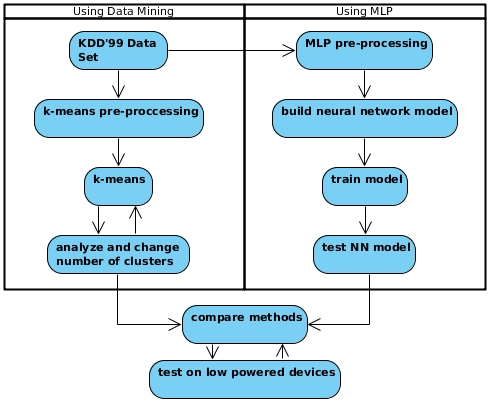
\includegraphics{methodology}
            \caption{Flow diagram of actions to be performed}
        \end{figure}


        \subsection{K-Means}
        \paragraph{}
        The goal of this work is to minimize computational load as much as possible. Therefore, while training and testing the datasets, it has been assumed that classifying an attack as an attack has more priority than classifying which type of attack the data packet resembles. This allowed the use of a minimum of 2 clusters for K-Means, one for attacks, the other for normal data. Luckily, the dataset has already been labeled in this manner as its 49th feature (label), which may be used for training and testing.

        \subsection{Multilayer Perceptron}
        \paragraph{}
        It has been seen that, to minimize computational load in a neural network, binarizing the weights is possible, at the cost of accuracy of prediction \cite{mlp17}. This attempt shall be made and analyzed with different configurations of hidden layers.

        \subsection{Performance Paramters}
        4 generic paramters will be used for comparing the two algorithms:
        \begin{itemize}
            \item True Positive (TP): Number of correctly classified attack records
            \item True Negative (TN): Number of correctly classified normal records
            \item False Positive (FP): Number of misclassified attack records
            \item False Negative (FN): Number of misclassified normal records
        \end{itemize}
        Using these 4 paramters, the accuracy may be calculated as:
        \begin{equation}
            accuracy = \frac {TP + TN} {TP + TN + FP + FN}
        \end{equation}

	\section{Work done so far}
        \subsection{Dataset}
        The choice of dataset was between 2 very popular ones used for testing IDSs, the KDD'99 and UNSW-NB15. Initial tests were run on the KDD'99, however, it had many problems as stated in \cite{unsw15}. As a result, another, more modern data set called UNSW-NB15, also used for IDS performance testing, was used. The dataset is much larger and carefully chosen training and testing data sets are available at their website. Te data set is modern and goes well with the present standards and tackles most of the issues of KDD’99, and has proven to be a beter performer according to \cite{unsw15}.
        \subsection{Pre-processing}
        The pre-processing of the dataset has been done using pandas library for python, following the steps mentioned in section 6.2. Figure 2 shows the results of running the script for preprocessing the data in an ipython terminal.
        \begin{figure}
            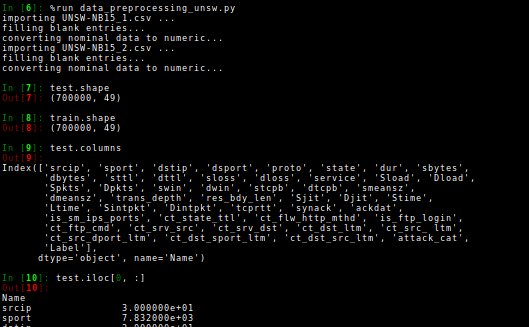
\includegraphics[width=1\textwidth]{preprocessing}
            \caption{Preprocessing the UNSW-NB15 dataset using part 1 as training set and part 2 as test set.}
        \end{figure}
        \subsection{K-Means}
        The execution of K-Means algorithm was done using 2 clusters to achieve an accuracy of 52.97\%. The algorithm needs ot be further optimized further to achieve more acceptable results. In 700,000 records, the model detected 327,461 TN, 9,399 FN, 319,790 FP and 43,350 FN. The results are shown in Figure 3. It is clear from the results that in anomaly based IDSs, the false positive rate is very high that has a major contribution in reducing the accuracy of the system.
        \begin{figure}
            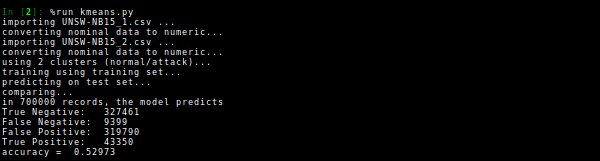
\includegraphics[width=1\textwidth]{kmeans}
            \caption{Results of running k-means on UNSW-NB15}
        \end{figure}

    \section{Remaining work}
        The following work has to done with their target dates:
        \begin{itemize}
            \item 20 Mar 2018: Implement MLP on the basis of \cite{mlp17} on UNSW-NB-15. More reading on this subject is required to understand the basis on which the number of layers are chosen.
            \item 25 Mar 2018: Analyze and compare the two algorithms on regular devices. This is important to set a benchmark score for the two algorithms for when tested on low powered devices. A correct parameter for deciding the efficiency of the algorithm must be defined on the basis of compute power and time spent on performing these algorithm, while taking their accuracy into account.
            \item 30 Mar 2018: Test on low powered devices to understand the feasibility of these systems on such devices.
            \item 15 Apr 2018: Make an attempt to scale down algorithms for low powered devices.
            \item 01 May 2018: Re-run tests and understand pros and cons of scaling down.
        \end{itemize}

	%References
	\bibliographystyle{IEEEtran}
	\bibliography{references}
	\end{document}
